%--------------------
% Packages
% -------------------
\documentclass[11pt,a4paper]{article}
\usepackage[utf8x]{inputenc}
\usepackage[T1]{fontenc}
%\usepackage{gentium}
\usepackage{mathptmx} % Use Times Font
\usepackage{amsmath}

\usepackage[pdftex]{graphicx} % Required for including pictures
\graphicspath{ {images/} }
\usepackage[swedish]{babel} % Swedish translations
\usepackage[pdftex,linkcolor=black,pdfborder={0 0 0}]{hyperref} % Format links for pdf
\usepackage{calc} % To reset the counter in the document after title page
\usepackage{enumitem} % Includes lists

\frenchspacing % No double spacing between sentences
\linespread{1.2} % Set linespace
\usepackage[a4paper, lmargin=0.1666\paperwidth, rmargin=0.1666\paperwidth, tmargin=0.1111\paperheight, bmargin=0.1111\paperheight]{geometry} %margins
%\usepackage{parskip}

\usepackage[all]{nowidow} % Tries to remove widows
\usepackage[protrusion=true,expansion=true]{microtype} % Improves typography, load after fontpackage is selected

\counterwithin*{subsection}{section}
\renewcommand{\thesubsection}{\thesection.\alph{subsection}}

%-----------------------
% Set pdf information and add title, fill in the fields
%-----------------------


\hypersetup{ 	
pdfsubject = {Machine Learning 2 - Final Assignment},
pdftitle = {Machine Learning 2 - Final Assignment},
pdfauthor = {Frans de Boer}
}

\title{Machine learning 2 - Final Assignment}

\author{
    Frans de Boer \\
    frans.deboer \\
    5661439 \\
}

%-----------------------
% Begin document
%-----------------------
\begin{document} %All text i dokumentet hamnar mellan dessa taggar, allt ovanför är formatering av dokumentet
\maketitle

The git repository for this assignment (including code and the report) can be found at github.com. I will make this repository public after the Brightspace deadline has passed.

\section{PAC Learning}

\subsection{Extend the proof that was given in the slides for the PAC-learnability of hyper-rectangles:
show that axis-aligned hyper-rectangles in n-dimensional feature spaces (n > 2) are PAC
learnable.}
  
We can extend the proof by taking the number of sides/faces of the hyper-rectangle into account.
\begin{itemize}
    \item A hyper-rectangle in 2-dimensional space is simply a rectangle and has 4 sides.
    \item A hyper-rectangle in 3-dimensional space is a rectangular box and has 6 sides.
\end{itemize}
For now I will assume the number of sides on a n-dimensional hyper-rectangle to be $F(n)$, and I will get back later to the calculation of $F(n)$.

To start we can follow the steps from the lecture. We have the ground truth n-dimensional hyper-rectangle $R$, and the current tightest fit rectangle $R'$. The error ($R - R'$) can be split into $F(n)$ strips $T'$. On each of these strips we can now grow a new strip $T$ such that the probability mass of $T$ is $\frac{\epsilon}{F(n)}$.

If $T$ covers $T'$ for all strips then the probability of an error is
\begin{equation}
    \label{eq:total_error}
    P[error] \leq \sum_{i=0}^{F(n)-1}P[T_i] = F(n)\frac{\epsilon}{F(n)} = \epsilon
\end{equation}

We can now estimate the probability that $T$ does not cover $T'$

\begin{align*} 
    &P[\textit{random x hits T}] = \frac{\epsilon}{F(n)} \\
    &P[\textit{random x misses T}] = 1 - \frac{\epsilon}{F(n)} \\
    &P[\textit{m random x's misses T}] = (1 - \frac{\epsilon}{F(n)})^m \\
\end{align*}

Since we have $F(n)$ strips:
\begin{align*} 
    &P[\textit{m random x's miss any Ts}] \leq F(n) (1 - \frac{\epsilon}{F(n)})^m \\
    &P[\textit{R' has larger error than } \epsilon] \leq F(n) (1 - \frac{\epsilon}{F(n)})^m\ < \delta \\
\end{align*}

Bounding the chance that our R' has an error larger than $\epsilon$ by $\delta$:

\[F(n) (1 - \frac{\epsilon}{F(n)})^m\ < \delta\]
Using $e^{-x} \geq (1-x)$
\[F(n)e^{-m\epsilon / F(n)} \geq F(n)(1 - \frac{\epsilon}{F(n)})^m\]
So instead we can use:

\begin{align*} 
    &F(n)e^{-m\epsilon / F(n)} < \delta \\ 
    &-m\epsilon / F(n) < \log{(\delta / F(n))} \\
    &m\epsilon / F(n) > \log{(F(n) / \delta)} \\
    &m > (F(n) / \epsilon)\log{(F(n) / \delta)} \\
\end{align*}

So any n-dimensional hyper-rectangle is learnable.

\subsection{Assume we have a 2-dimensional feature space R2, and consider the set of concepts that are L1-balls: $c = \{(x, y) : |x| + |y| ≤ r\}$ (basically, all L1-balls centered around the origin). Use a learner that fits the tightest ball. Show that this class is PAC-learnable from training data of size m.}

Same thing? what. literally just question a but now rotated 45 degrees

\subsection{Now we extend the previous class by allowing the varying center: $c = \{(x, y) : |x − x0| + |y − y0| ≤ r\}$. Is this class PAC-learnable? Proof if it is, or otherwise disproof it.}

maybe, maybe not. can't you still just do the tightest fit L1 ball?
consistent learner so PAC learnable?

\clearpage
\section{VC Dimension}
\label{sec:VC}
Let us assume we are dealing with a two-class classification problem in d-dimensions.
Let us start off with refreshing our memories. Consider the class of linear hypotheses (i.e.,
all possible linear classifiers) in d-dimensional space.

\subsection{Given N data points, how many possible labelings does this data set have?}
\label{sec:2a}
Each data point can have 2 labels, so $2^n$

\subsection{What is the dimensionality d we need, at the least, for our class of linear hypotheses to
be able to find perfect solutions to all possible labelings of a data set of size N? Stated
differently, what is the smallest d that allows us to shatter N points?}
\label{sec:2b}
$d - 1$ 


\subsection{Consider d = 1 and a data set of size N. At maximum, how many different labelings of
such a data set can decision stumps solve perfectly, i.e., with zero training error?}
\label{sec:2c}
This would be all cases where there is no overlap, i.e. all points with class 1 (or 2) are either all on the left or right side. See Figure \ref{fig:stump} for an example with N=3. Note that the first 3 and last 3 examples are the same, just with inverted labelings.

\begin{figure}[h]
    \caption{Example of perfectly solvable labels with $N=3$}
    \centering
    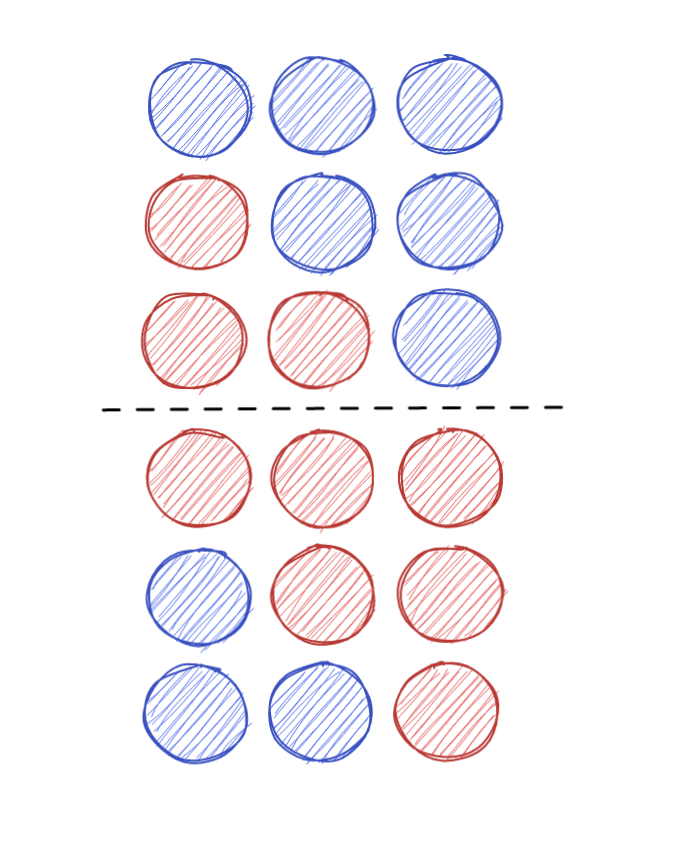
\includegraphics[width=0.5\textwidth]{stump.png}
    \label{fig:stump}
\end{figure}

With a dataset of size N, there are N ways in which we can have class 1 be on the left side and have a decision stump be able to solve it perfectly. There can be $1, 2, ..., N$ points with class 1 in a row.
Because each of these possible label assignments has a compliment (just invert the classes), we end up with a total of $2N$ possible labelings that a decision stump can solve perfectly.

\subsection{With the answer from 3.c, give an upper-bound on the maximum number of different
labelings a data set of size N in d dimensions can get by means of decision stumps.}
\label{sec:2d}

We can once again look at Figure \ref*{fig:stump}, but now instead of true labels we can view the labels (red and blue) as labels predicted by the decision stump. The decision stump either assigns all points to the left of it as class 1 or as class 2. So in $d=1$ we know the maximum number of different labelings a data set of size N can get is $2N$. 

Now to generalize this case to any dimension $d$. A possible problem with higher dimension spaces is that not each stump can shatter all N points. See Figure \ref{fig:non-shatter-stump} as an example. Since we are looking for the upper bound from now on I will make the assumption that the data set can be shattered, i.e. for $d=2$
$$x_i \neq x_j \land y_i \neq y_j \forall i,j$$
See Figure \ref{fig:shatter-stump} for an example.

\begin{figure}[h]
    \caption{Example of dataset that can't be shattered by a stump in $d=2$}
    \centering
    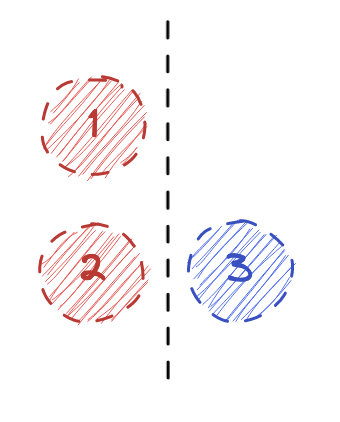
\includegraphics[width=0.5\textwidth]{non-shatter-stump.png}
    \label{fig:non-shatter-stump}
\end{figure}

\begin{figure}[h]
    \caption{Example of dataset that can be shattered by a stump in $d=2$}
    \centering
    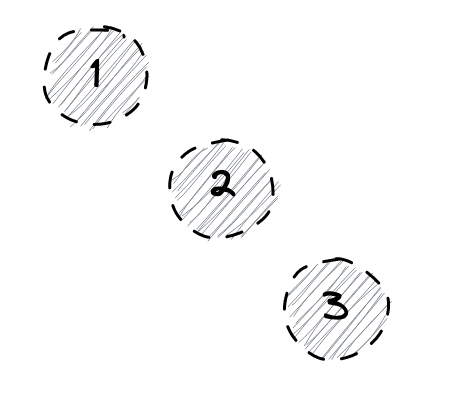
\includegraphics[width=0.5\textwidth]{shatter-stump.png}
    \label{fig:shatter-stump}
\end{figure}

A stump can only choose 1 variable (dimension) to make its decision. This means that per variable a stump can create $2N$ possible labelings (Section \ref{sec:2c}). In $d$ dimensions we can create $d$ possible stumps, so in total there are $2Nd$ possible labelings.

So the upper-bound on the maximum number of different labels a data set of size $N$ in $d$ dimensions can get by means of decision stumps is $2Nd$. 

\subsection{Using the bound from Exercise 3.d, determine the smallest upper-bound on the VC-dimension for decision stumps for dimensionalities $d ∈ \{1, 2, 3, 4, 5, 6, 7, 8, 1024, 2100\}$}
\label{sec:3e}
\textbf{VC-Dimension}: The largest number of nodes $N$ that a classifier can shatter in all possible $2^N$ ways.

in d=1 2? in d=2 2?

\end{document}